\begin{enumerate}
    \item Consider the logic circuit
    \begin{center}
    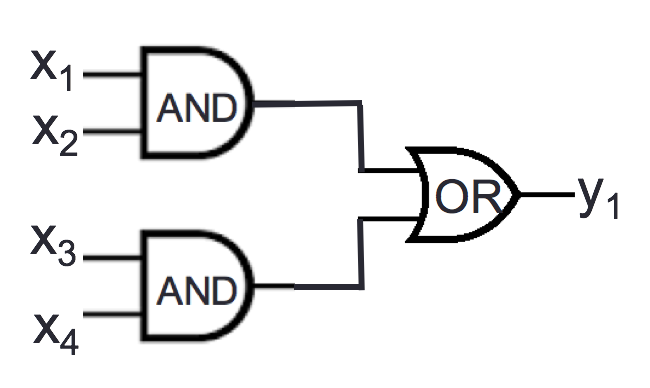
\includegraphics[width=2in]{../resources/images/review-circuit-3.png}
    \end{center}
    For which of the following settings(s) of input values is the output
    $y_1 =  0$? (Select all and only those that apply.)
    \begin{enumerate}
        \item $x_1 = 0$, $x_2 = 0$, $x_3 = 0$, and $x_4 = 0$
        \item $x_1 = 1$, $x_2 = 1$, $x_3 = 1$, and $x_4 = 1$
        \item $x_1 = 1$, $x_2 = 0$, $x_3 = 0$, and $x_4 = 1$
        \item $x_1 = 0$, $x_2 = 0$, $x_3 = 1$, and $x_4 = 1$
    \end{enumerate}
    \item Consider the logic circuits
    \begin{center}
    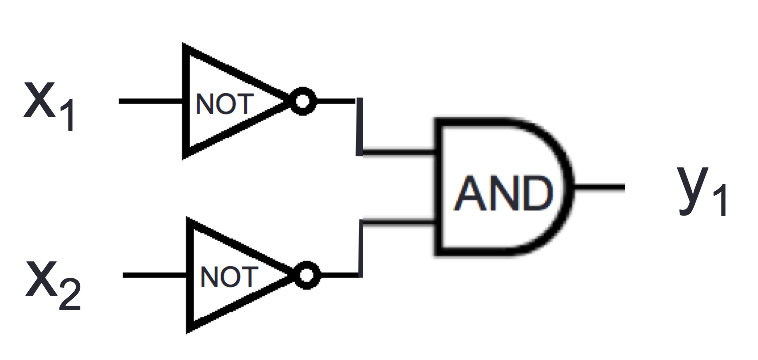
\includegraphics[width=2in]{../resources/images/review-circuit-1.png}
    \qquad \qquad \qquad
    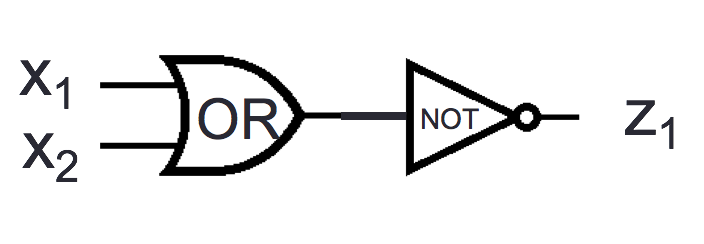
\includegraphics[width=2in]{../resources/images/review-circuit-4.png}
    \end{center}
    For which  of the following settings(s) of input values do the outputs
    of these  circuits have the  same value, i.e.\ $y_1 =  z_1$? 
    (Select all and only those that apply.)
    \begin{enumerate}
        \item $x_1 = 1$, $x_2 = 1$
        \item $x_1 = 1$, $x_2 = 0$
        \item $x_1 = 0$, $x_2 = 1$
        \item $x_1 = 0$, $x_2 = 0$
    \end{enumerate}    
    
\end{enumerate}